% Options for packages loaded elsewhere
\PassOptionsToPackage{unicode}{hyperref}
\PassOptionsToPackage{hyphens}{url}
%
\documentclass[
]{article}
\usepackage{amsmath,amssymb}
\usepackage{iftex}
\ifPDFTeX
  \usepackage[T1]{fontenc}
  \usepackage[utf8]{inputenc}
  \usepackage{textcomp} % provide euro and other symbols
\else % if luatex or xetex
  \usepackage{unicode-math} % this also loads fontspec
  \defaultfontfeatures{Scale=MatchLowercase}
  \defaultfontfeatures[\rmfamily]{Ligatures=TeX,Scale=1}
\fi
\usepackage{lmodern}
\ifPDFTeX\else
  % xetex/luatex font selection
\fi
% Use upquote if available, for straight quotes in verbatim environments
\IfFileExists{upquote.sty}{\usepackage{upquote}}{}
\IfFileExists{microtype.sty}{% use microtype if available
  \usepackage[]{microtype}
  \UseMicrotypeSet[protrusion]{basicmath} % disable protrusion for tt fonts
}{}
\makeatletter
\@ifundefined{KOMAClassName}{% if non-KOMA class
  \IfFileExists{parskip.sty}{%
    \usepackage{parskip}
  }{% else
    \setlength{\parindent}{0pt}
    \setlength{\parskip}{6pt plus 2pt minus 1pt}}
}{% if KOMA class
  \KOMAoptions{parskip=half}}
\makeatother
\usepackage{xcolor}
\usepackage[margin=1in]{geometry}
\usepackage{color}
\usepackage{fancyvrb}
\newcommand{\VerbBar}{|}
\newcommand{\VERB}{\Verb[commandchars=\\\{\}]}
\DefineVerbatimEnvironment{Highlighting}{Verbatim}{commandchars=\\\{\}}
% Add ',fontsize=\small' for more characters per line
\usepackage{framed}
\definecolor{shadecolor}{RGB}{248,248,248}
\newenvironment{Shaded}{\begin{snugshade}}{\end{snugshade}}
\newcommand{\AlertTok}[1]{\textcolor[rgb]{0.94,0.16,0.16}{#1}}
\newcommand{\AnnotationTok}[1]{\textcolor[rgb]{0.56,0.35,0.01}{\textbf{\textit{#1}}}}
\newcommand{\AttributeTok}[1]{\textcolor[rgb]{0.13,0.29,0.53}{#1}}
\newcommand{\BaseNTok}[1]{\textcolor[rgb]{0.00,0.00,0.81}{#1}}
\newcommand{\BuiltInTok}[1]{#1}
\newcommand{\CharTok}[1]{\textcolor[rgb]{0.31,0.60,0.02}{#1}}
\newcommand{\CommentTok}[1]{\textcolor[rgb]{0.56,0.35,0.01}{\textit{#1}}}
\newcommand{\CommentVarTok}[1]{\textcolor[rgb]{0.56,0.35,0.01}{\textbf{\textit{#1}}}}
\newcommand{\ConstantTok}[1]{\textcolor[rgb]{0.56,0.35,0.01}{#1}}
\newcommand{\ControlFlowTok}[1]{\textcolor[rgb]{0.13,0.29,0.53}{\textbf{#1}}}
\newcommand{\DataTypeTok}[1]{\textcolor[rgb]{0.13,0.29,0.53}{#1}}
\newcommand{\DecValTok}[1]{\textcolor[rgb]{0.00,0.00,0.81}{#1}}
\newcommand{\DocumentationTok}[1]{\textcolor[rgb]{0.56,0.35,0.01}{\textbf{\textit{#1}}}}
\newcommand{\ErrorTok}[1]{\textcolor[rgb]{0.64,0.00,0.00}{\textbf{#1}}}
\newcommand{\ExtensionTok}[1]{#1}
\newcommand{\FloatTok}[1]{\textcolor[rgb]{0.00,0.00,0.81}{#1}}
\newcommand{\FunctionTok}[1]{\textcolor[rgb]{0.13,0.29,0.53}{\textbf{#1}}}
\newcommand{\ImportTok}[1]{#1}
\newcommand{\InformationTok}[1]{\textcolor[rgb]{0.56,0.35,0.01}{\textbf{\textit{#1}}}}
\newcommand{\KeywordTok}[1]{\textcolor[rgb]{0.13,0.29,0.53}{\textbf{#1}}}
\newcommand{\NormalTok}[1]{#1}
\newcommand{\OperatorTok}[1]{\textcolor[rgb]{0.81,0.36,0.00}{\textbf{#1}}}
\newcommand{\OtherTok}[1]{\textcolor[rgb]{0.56,0.35,0.01}{#1}}
\newcommand{\PreprocessorTok}[1]{\textcolor[rgb]{0.56,0.35,0.01}{\textit{#1}}}
\newcommand{\RegionMarkerTok}[1]{#1}
\newcommand{\SpecialCharTok}[1]{\textcolor[rgb]{0.81,0.36,0.00}{\textbf{#1}}}
\newcommand{\SpecialStringTok}[1]{\textcolor[rgb]{0.31,0.60,0.02}{#1}}
\newcommand{\StringTok}[1]{\textcolor[rgb]{0.31,0.60,0.02}{#1}}
\newcommand{\VariableTok}[1]{\textcolor[rgb]{0.00,0.00,0.00}{#1}}
\newcommand{\VerbatimStringTok}[1]{\textcolor[rgb]{0.31,0.60,0.02}{#1}}
\newcommand{\WarningTok}[1]{\textcolor[rgb]{0.56,0.35,0.01}{\textbf{\textit{#1}}}}
\usepackage{graphicx}
\makeatletter
\def\maxwidth{\ifdim\Gin@nat@width>\linewidth\linewidth\else\Gin@nat@width\fi}
\def\maxheight{\ifdim\Gin@nat@height>\textheight\textheight\else\Gin@nat@height\fi}
\makeatother
% Scale images if necessary, so that they will not overflow the page
% margins by default, and it is still possible to overwrite the defaults
% using explicit options in \includegraphics[width, height, ...]{}
\setkeys{Gin}{width=\maxwidth,height=\maxheight,keepaspectratio}
% Set default figure placement to htbp
\makeatletter
\def\fps@figure{htbp}
\makeatother
\setlength{\emergencystretch}{3em} % prevent overfull lines
\providecommand{\tightlist}{%
  \setlength{\itemsep}{0pt}\setlength{\parskip}{0pt}}
\setcounter{secnumdepth}{-\maxdimen} % remove section numbering
\usepackage{booktabs}
\usepackage{longtable}
\usepackage{array}
\usepackage{multirow}
\usepackage{wrapfig}
\usepackage{float}
\usepackage{colortbl}
\usepackage{pdflscape}
\usepackage{tabu}
\usepackage{threeparttable}
\usepackage{threeparttablex}
\usepackage[normalem]{ulem}
\usepackage{makecell}
\usepackage{xcolor}
\ifLuaTeX
  \usepackage{selnolig}  % disable illegal ligatures
\fi
\usepackage{bookmark}
\IfFileExists{xurl.sty}{\usepackage{xurl}}{} % add URL line breaks if available
\urlstyle{same}
\hypersetup{
  pdftitle={Zip Competition},
  pdfauthor={Luana Lima},
  hidelinks,
  pdfcreator={LaTeX via pandoc}}

\title{Zip Competition}
\author{Luana Lima}
\date{}

\begin{document}
\maketitle

\begin{Shaded}
\begin{Highlighting}[]
\NormalTok{knitr}\SpecialCharTok{::}\NormalTok{opts\_chunk}\SpecialCharTok{$}\FunctionTok{set}\NormalTok{(}\AttributeTok{echo =} \ConstantTok{TRUE}\NormalTok{,}\AttributeTok{tidy.opts=}\FunctionTok{list}\NormalTok{(}\AttributeTok{width.cutoff=}\DecValTok{80}\NormalTok{), }\AttributeTok{tidy=}\ConstantTok{FALSE}\NormalTok{) }
\end{Highlighting}
\end{Shaded}

\begin{Shaded}
\begin{Highlighting}[]
\FunctionTok{library}\NormalTok{(lubridate)}
\end{Highlighting}
\end{Shaded}

\begin{verbatim}
## 
## Attaching package: 'lubridate'
\end{verbatim}

\begin{verbatim}
## The following objects are masked from 'package:base':
## 
##     date, intersect, setdiff, union
\end{verbatim}

\begin{Shaded}
\begin{Highlighting}[]
\FunctionTok{library}\NormalTok{(ggplot2)}
\FunctionTok{library}\NormalTok{(forecast)  }
\end{Highlighting}
\end{Shaded}

\begin{verbatim}
## Registered S3 method overwritten by 'quantmod':
##   method            from
##   as.zoo.data.frame zoo
\end{verbatim}

\begin{Shaded}
\begin{Highlighting}[]
\FunctionTok{library}\NormalTok{(Kendall)}
\FunctionTok{library}\NormalTok{(tseries)}
\FunctionTok{library}\NormalTok{(outliers)}
\FunctionTok{library}\NormalTok{(tidyverse)}
\end{Highlighting}
\end{Shaded}

\begin{verbatim}
## -- Attaching core tidyverse packages ------------------------ tidyverse 2.0.0 --
## v dplyr   1.1.4     v stringr 1.5.1
## v forcats 1.0.0     v tibble  3.2.1
## v purrr   1.0.2     v tidyr   1.3.1
## v readr   2.1.5
\end{verbatim}

\begin{verbatim}
## -- Conflicts ------------------------------------------ tidyverse_conflicts() --
## x dplyr::filter() masks stats::filter()
## x dplyr::lag()    masks stats::lag()
## i Use the conflicted package (<http://conflicted.r-lib.org/>) to force all conflicts to become errors
\end{verbatim}

\begin{Shaded}
\begin{Highlighting}[]
\FunctionTok{library}\NormalTok{(smooth)}
\end{Highlighting}
\end{Shaded}

\begin{verbatim}
## Loading required package: greybox
## Package "greybox", v2.0.8 loaded.
## 
## 
## Attaching package: 'greybox'
## 
## The following object is masked from 'package:tidyr':
## 
##     spread
## 
## The following object is masked from 'package:lubridate':
## 
##     hm
## 
## This is package "smooth", v4.4.0
\end{verbatim}

\begin{Shaded}
\begin{Highlighting}[]
\FunctionTok{library}\NormalTok{(zoo)}
\end{Highlighting}
\end{Shaded}

\begin{verbatim}
## 
## Attaching package: 'zoo'
## 
## The following objects are masked from 'package:base':
## 
##     as.Date, as.Date.numeric
\end{verbatim}

\begin{Shaded}
\begin{Highlighting}[]
\FunctionTok{library}\NormalTok{(kableExtra)}
\end{Highlighting}
\end{Shaded}

\begin{verbatim}
## 
## Attaching package: 'kableExtra'
## 
## The following object is masked from 'package:dplyr':
## 
##     group_rows
\end{verbatim}

\begin{Shaded}
\begin{Highlighting}[]
\NormalTok{tinytex}\SpecialCharTok{::}\FunctionTok{tlmgr\_install}\NormalTok{(}\StringTok{"multirow"}\NormalTok{)}
\end{Highlighting}
\end{Shaded}

\begin{verbatim}
## tlmgr install multirow
## tlmgr update --self
## A new version of TeX Live has been released. If you need to install or update any LaTeX packages, you have to upgrade TinyTeX with tinytex::reinstall_tinytex(repository = "illinois").
## tlmgr install multirow
\end{verbatim}

\#Import Data

\begin{Shaded}
\begin{Highlighting}[]
\FunctionTok{install.packages}\NormalTok{(}\StringTok{"readxl"}\NormalTok{)}
\end{Highlighting}
\end{Shaded}

\begin{verbatim}
## Installing package into '/home/guest/R/x86_64-pc-linux-gnu-library/4.4'
## (as 'lib' is unspecified)
\end{verbatim}

\begin{Shaded}
\begin{Highlighting}[]
\FunctionTok{library}\NormalTok{(readxl)}

\CommentTok{\#import load data }

\NormalTok{load }\OtherTok{\textless{}{-}} \FunctionTok{read\_excel}\NormalTok{(}\AttributeTok{path  =} \StringTok{"../Competition/load.xlsx"}\NormalTok{, }\AttributeTok{sheet =} \DecValTok{1}\NormalTok{, }\AttributeTok{col\_names =} \ConstantTok{TRUE}\NormalTok{)}
\FunctionTok{class}\NormalTok{(load}\SpecialCharTok{$}\NormalTok{date)}
\end{Highlighting}
\end{Shaded}

\begin{verbatim}
## [1] "POSIXct" "POSIXt"
\end{verbatim}

\begin{Shaded}
\begin{Highlighting}[]
\CommentTok{\#Convert to daily data}

\NormalTok{load\_daily }\OtherTok{\textless{}{-}}\NormalTok{ load }\SpecialCharTok{\%\textgreater{}\%}
  \FunctionTok{mutate}\NormalTok{(}\AttributeTok{date =} \FunctionTok{as.Date}\NormalTok{(date)) }\SpecialCharTok{\%\textgreater{}\%}                  
  \FunctionTok{mutate}\NormalTok{(}\AttributeTok{daily\_mean =} \FunctionTok{rowMeans}\NormalTok{(}\FunctionTok{select}\NormalTok{(., h1}\SpecialCharTok{:}\NormalTok{h24), }
                               \AttributeTok{na.rm =} \ConstantTok{TRUE}\NormalTok{)) }\SpecialCharTok{\%\textgreater{}\%}
  \FunctionTok{select}\NormalTok{(meter\_id, date, daily\_mean) }

\CommentTok{\#Convert to time series}
\NormalTok{load\_ts }\OtherTok{\textless{}{-}} \FunctionTok{msts}\NormalTok{(load\_daily}\SpecialCharTok{$}\NormalTok{daily\_mean,}
                \AttributeTok{seasonal.periods =} \FunctionTok{c}\NormalTok{(}\DecValTok{7}\NormalTok{, }\FloatTok{365.25}\NormalTok{),}
                \AttributeTok{start =} \FunctionTok{c}\NormalTok{(}\DecValTok{2005}\NormalTok{, }\DecValTok{1}\NormalTok{))}
\end{Highlighting}
\end{Shaded}

\#Train the model

\begin{Shaded}
\begin{Highlighting}[]
\CommentTok{\#Use data from January 1, 2005, to July 31, 2010}

\NormalTok{load\_daily\_2010July }\OtherTok{\textless{}{-}}\NormalTok{ load\_daily }\SpecialCharTok{\%\textgreater{}\%}
  \FunctionTok{filter}\NormalTok{(date }\SpecialCharTok{\textless{}=} \FunctionTok{as.Date}\NormalTok{(}\StringTok{"2010{-}07{-}31"}\NormalTok{))}

\NormalTok{load\_daily\_2010July }\OtherTok{\textless{}{-}} \FunctionTok{msts}\NormalTok{(load\_daily\_2010July}\SpecialCharTok{$}\NormalTok{daily\_mean,}
                     \AttributeTok{seasonal.periods =} \FunctionTok{c}\NormalTok{(}\DecValTok{7}\NormalTok{, }\FloatTok{365.25}\NormalTok{),}
                     \AttributeTok{start =} \FunctionTok{c}\NormalTok{(}\DecValTok{2005}\NormalTok{, }\DecValTok{1}\NormalTok{))}
\NormalTok{n\_for }\OtherTok{\textless{}{-}} \DecValTok{31}

\CommentTok{\#Train the data}
\NormalTok{load\_ts\_train }\OtherTok{\textless{}{-}} \FunctionTok{subset}\NormalTok{(load\_daily\_2010July, }\AttributeTok{end =} \FunctionTok{length}\NormalTok{(load\_daily\_2010July) }\SpecialCharTok{{-}}\NormalTok{ n\_for)}

\CommentTok{\#Test}
\NormalTok{load\_ts\_test  }\OtherTok{\textless{}{-}} \FunctionTok{subset}\NormalTok{(load\_daily\_2010July, }\AttributeTok{start =} \FunctionTok{length}\NormalTok{(load\_daily\_2010July) }\SpecialCharTok{{-}}\NormalTok{ n\_for }\SpecialCharTok{+} \DecValTok{1}\NormalTok{)}

\FunctionTok{autoplot}\NormalTok{(load\_ts\_train)}
\end{Highlighting}
\end{Shaded}

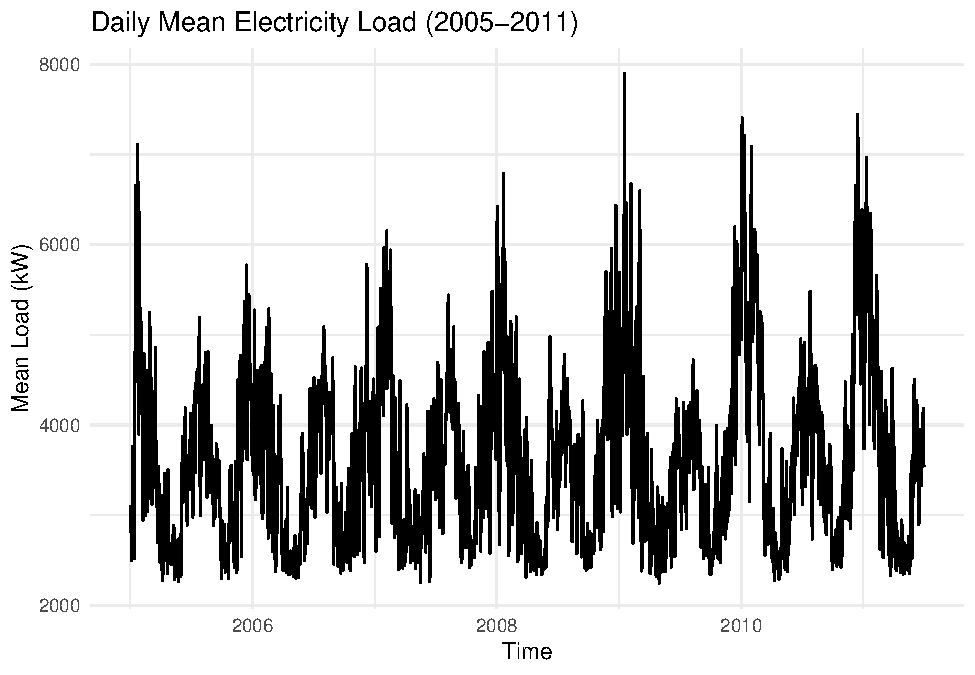
\includegraphics{Pang_Zhang_FirstSubmission_files/figure-latex/unnamed-chunk-4-1.pdf}

\begin{Shaded}
\begin{Highlighting}[]
\FunctionTok{autoplot}\NormalTok{(load\_ts\_test)}
\end{Highlighting}
\end{Shaded}

\includegraphics{Pang_Zhang_FirstSubmission_files/figure-latex/unnamed-chunk-4-2.pdf}

Model 1 Naive Model

Step 1 Test and Record Score

\begin{Shaded}
\begin{Highlighting}[]
\NormalTok{SNAIVE\_test }\OtherTok{\textless{}{-}} \FunctionTok{snaive}\NormalTok{(load\_ts\_train, }\AttributeTok{h =}\NormalTok{ n\_for, }\AttributeTok{holdout =} \ConstantTok{FALSE}\NormalTok{)}
\NormalTok{SNAIVE\_scores}\OtherTok{\textless{}{-}} \FunctionTok{accuracy}\NormalTok{(SNAIVE\_test}\SpecialCharTok{$}\NormalTok{mean, load\_ts\_test)}
\end{Highlighting}
\end{Shaded}

Model 2: TBATS

Step 1: Test and Record Score

\begin{Shaded}
\begin{Highlighting}[]
\CommentTok{\# Test TBATS}
\NormalTok{TBATS\_fit }\OtherTok{\textless{}{-}} \FunctionTok{tbats}\NormalTok{(load\_ts\_train)}
\NormalTok{TBATS\_for }\OtherTok{\textless{}{-}} \FunctionTok{forecast}\NormalTok{(TBATS\_fit, }\AttributeTok{h =}\NormalTok{ n\_for)}
\NormalTok{TBATS\_scores }\OtherTok{\textless{}{-}} \FunctionTok{accuracy}\NormalTok{(TBATS\_for}\SpecialCharTok{$}\NormalTok{mean, load\_ts\_test)}
\end{Highlighting}
\end{Shaded}

Step 2 Compare

\begin{Shaded}
\begin{Highlighting}[]
\CommentTok{\# Compare with Naive Model}
\NormalTok{scores }\OtherTok{\textless{}{-}} \FunctionTok{as.data.frame}\NormalTok{(}\FunctionTok{rbind}\NormalTok{(SNAIVE\_scores, TBATS\_scores))}
\FunctionTok{row.names}\NormalTok{(scores) }\OtherTok{\textless{}{-}} \FunctionTok{c}\NormalTok{(}\StringTok{"SNAIVE"}\NormalTok{, }\StringTok{"TBATS"}\NormalTok{)}
\FunctionTok{print}\NormalTok{(scores)}
\end{Highlighting}
\end{Shaded}

\begin{verbatim}
##               ME     RMSE      MAE       MPE     MAPE      ACF1 Theil's U
## SNAIVE 606.47849 950.3533 837.1102 12.348224 19.35913 0.4370708  1.772924
## TBATS  -37.89045 578.1685 444.7257 -3.010307 11.34223 0.4591482  1.132356
\end{verbatim}

Model 3 STL+ETS

Step 1: Test and Record Score

\begin{Shaded}
\begin{Highlighting}[]
\NormalTok{ETS\_fit }\OtherTok{\textless{}{-}} \FunctionTok{stlf}\NormalTok{(load\_ts\_train, }\AttributeTok{h =}\NormalTok{ n\_for)}
\NormalTok{ETS\_scores }\OtherTok{\textless{}{-}} \FunctionTok{accuracy}\NormalTok{(ETS\_fit}\SpecialCharTok{$}\NormalTok{mean, load\_ts\_test)}
\end{Highlighting}
\end{Shaded}

Step 2 Compare

\begin{Shaded}
\begin{Highlighting}[]
\CommentTok{\# Compare}
\NormalTok{scores }\OtherTok{\textless{}{-}} \FunctionTok{as.data.frame}\NormalTok{(}\FunctionTok{rbind}\NormalTok{(SNAIVE\_scores, TBATS\_scores, ETS\_scores))}
\FunctionTok{row.names}\NormalTok{(scores) }\OtherTok{\textless{}{-}} \FunctionTok{c}\NormalTok{(}\StringTok{"SNAIVE"}\NormalTok{, }\StringTok{"TBATS"}\NormalTok{, }\StringTok{"STL+ETS"}\NormalTok{)}
\FunctionTok{print}\NormalTok{(scores)}
\end{Highlighting}
\end{Shaded}

\begin{verbatim}
##                ME     RMSE      MAE       MPE     MAPE      ACF1 Theil's U
## SNAIVE  606.47849 950.3533 837.1102 12.348224 19.35913 0.4370708  1.772924
## TBATS   -37.89045 578.1685 444.7257 -3.010307 11.34223 0.4591482  1.132356
## STL+ETS 168.52289 705.1976 590.3347  1.701303 14.49321 0.5152893  1.339416
\end{verbatim}

\begin{quote}
TBATS has the best result.
\end{quote}

Model 4: Neural Network

\begin{Shaded}
\begin{Highlighting}[]
\NormalTok{NN\_fit }\OtherTok{\textless{}{-}} \FunctionTok{nnetar}\NormalTok{(load\_ts\_train,}
                 \AttributeTok{p =} \DecValTok{7}\NormalTok{,}
                 \AttributeTok{P =} \DecValTok{1}\NormalTok{,}
                 \AttributeTok{xreg =} \FunctionTok{fourier}\NormalTok{(load\_ts\_train, }\AttributeTok{K =} \FunctionTok{c}\NormalTok{(}\DecValTok{2}\NormalTok{, }\DecValTok{2}\NormalTok{)))}

\NormalTok{NN\_for }\OtherTok{\textless{}{-}} \FunctionTok{forecast}\NormalTok{(NN\_fit,}
                   \AttributeTok{h =}\NormalTok{ n\_for,}
                   \AttributeTok{xreg =} \FunctionTok{fourier}\NormalTok{(load\_ts\_train, }\AttributeTok{K =} \FunctionTok{c}\NormalTok{(}\DecValTok{2}\NormalTok{, }\DecValTok{2}\NormalTok{), }\AttributeTok{h =}\NormalTok{ n\_for))}

\NormalTok{NN\_scores }\OtherTok{\textless{}{-}} \FunctionTok{accuracy}\NormalTok{(NN\_for}\SpecialCharTok{$}\NormalTok{mean, load\_ts\_test)}
\end{Highlighting}
\end{Shaded}

Model 5: STL+ARIMA

\begin{Shaded}
\begin{Highlighting}[]
\CommentTok{\# Model 5: STL + ARIMA}
\NormalTok{STLARIMA\_fit }\OtherTok{\textless{}{-}} \FunctionTok{stlf}\NormalTok{(load\_ts\_train, }\AttributeTok{method =} \StringTok{"arima"}\NormalTok{, }\AttributeTok{h =}\NormalTok{ n\_for)}
\NormalTok{STLARIMA\_scores }\OtherTok{\textless{}{-}} \FunctionTok{accuracy}\NormalTok{(STLARIMA\_fit}\SpecialCharTok{$}\NormalTok{mean, load\_ts\_test)}
\FunctionTok{print}\NormalTok{(STLARIMA\_scores)}
\end{Highlighting}
\end{Shaded}

\begin{verbatim}
##                ME     RMSE      MAE       MPE     MAPE      ACF1 Theil's U
## Test set 3.661967 684.0319 554.8278 -2.301434 14.07411 0.5121983  1.344091
\end{verbatim}

Model 6: ARIMA

\begin{Shaded}
\begin{Highlighting}[]
\CommentTok{\# Model 6: ARIMA + Fourier}
\NormalTok{ARIMA\_Four\_fit }\OtherTok{\textless{}{-}} \FunctionTok{Arima}\NormalTok{(load\_ts\_train,}
                        \AttributeTok{order =} \FunctionTok{c}\NormalTok{(}\DecValTok{2}\NormalTok{, }\DecValTok{0}\NormalTok{, }\DecValTok{1}\NormalTok{),}
                        \AttributeTok{xreg =} \FunctionTok{fourier}\NormalTok{(load\_ts\_train, }\AttributeTok{K =} \FunctionTok{c}\NormalTok{(}\DecValTok{2}\NormalTok{, }\DecValTok{6}\NormalTok{)))}
\NormalTok{ARIMA\_Four\_for }\OtherTok{\textless{}{-}} \FunctionTok{forecast}\NormalTok{(ARIMA\_Four\_fit,}
                           \AttributeTok{h =}\NormalTok{ n\_for,}
                           \AttributeTok{xreg =} \FunctionTok{fourier}\NormalTok{(load\_ts\_train, }\AttributeTok{K =} \FunctionTok{c}\NormalTok{(}\DecValTok{2}\NormalTok{, }\DecValTok{6}\NormalTok{), }\AttributeTok{h =}\NormalTok{ n\_for))}

\NormalTok{ARIMA\_Four\_scores }\OtherTok{\textless{}{-}} \FunctionTok{accuracy}\NormalTok{(ARIMA\_Four\_for}\SpecialCharTok{$}\NormalTok{mean, load\_ts\_test)}
\FunctionTok{print}\NormalTok{(ARIMA\_Four\_scores)}
\end{Highlighting}
\end{Shaded}

\begin{verbatim}
##                ME     RMSE      MAE      MPE    MAPE      ACF1 Theil's U
## Test set 332.3217 671.9644 553.1793 5.955252 12.9342 0.4704854  1.224464
\end{verbatim}

\begin{Shaded}
\begin{Highlighting}[]
\CommentTok{\# Different K}
\NormalTok{ARIMA\_Four\_fit2 }\OtherTok{\textless{}{-}} \FunctionTok{Arima}\NormalTok{(load\_ts\_train,}
                         \AttributeTok{order =} \FunctionTok{c}\NormalTok{(}\DecValTok{2}\NormalTok{, }\DecValTok{0}\NormalTok{, }\DecValTok{1}\NormalTok{),}
                         \AttributeTok{xreg =} \FunctionTok{fourier}\NormalTok{(load\_ts\_train, }\AttributeTok{K =} \FunctionTok{c}\NormalTok{(}\DecValTok{3}\NormalTok{, }\DecValTok{8}\NormalTok{)))}

\NormalTok{ARIMA\_Four\_for2 }\OtherTok{\textless{}{-}} \FunctionTok{forecast}\NormalTok{(ARIMA\_Four\_fit2,}
                            \AttributeTok{h =}\NormalTok{ n\_for,}
                            \AttributeTok{xreg =} \FunctionTok{fourier}\NormalTok{(load\_ts\_train, }\AttributeTok{K =} \FunctionTok{c}\NormalTok{(}\DecValTok{3}\NormalTok{, }\DecValTok{8}\NormalTok{), }\AttributeTok{h =}\NormalTok{ n\_for))}

\NormalTok{ARIMA\_Four\_scores2 }\OtherTok{\textless{}{-}} \FunctionTok{accuracy}\NormalTok{(ARIMA\_Four\_for2}\SpecialCharTok{$}\NormalTok{mean, load\_ts\_test)}
\FunctionTok{print}\NormalTok{(ARIMA\_Four\_scores2)}
\end{Highlighting}
\end{Shaded}

\begin{verbatim}
##                ME     RMSE      MAE      MPE     MAPE      ACF1 Theil's U
## Test set 327.6127 668.2723 549.9488 5.868703 12.88309 0.4614754    1.2199
\end{verbatim}

Combo: TBATS + NN

\begin{Shaded}
\begin{Highlighting}[]
\CommentTok{\# Combination: TBATS + NN}
\NormalTok{COMBO\_for }\OtherTok{\textless{}{-}}\NormalTok{ (TBATS\_for}\SpecialCharTok{$}\NormalTok{mean }\SpecialCharTok{+}\NormalTok{ NN\_for}\SpecialCharTok{$}\NormalTok{mean) }\SpecialCharTok{/} \DecValTok{2}
\NormalTok{COMBO\_scores }\OtherTok{\textless{}{-}} \FunctionTok{accuracy}\NormalTok{(COMBO\_for, load\_ts\_test)}
\FunctionTok{print}\NormalTok{(COMBO\_scores)}
\end{Highlighting}
\end{Shaded}

\begin{verbatim}
##                ME   RMSE      MAE      MPE     MAPE      ACF1 Theil's U
## Test set 174.4403 598.28 482.5254 2.143448 11.64323 0.4812458  1.110593
\end{verbatim}

\begin{Shaded}
\begin{Highlighting}[]
\CommentTok{\# More weight on TBATS}
\NormalTok{COMBO2\_for }\OtherTok{\textless{}{-}}\NormalTok{ (TBATS\_for}\SpecialCharTok{$}\NormalTok{mean }\SpecialCharTok{*} \FloatTok{0.7} \SpecialCharTok{+}\NormalTok{ NN\_for}\SpecialCharTok{$}\NormalTok{mean }\SpecialCharTok{*} \FloatTok{0.3}\NormalTok{)}
\NormalTok{COMBO2\_scores }\OtherTok{\textless{}{-}} \FunctionTok{accuracy}\NormalTok{(COMBO2\_for, load\_ts\_test)}
\FunctionTok{print}\NormalTok{(COMBO2\_scores)}
\end{Highlighting}
\end{Shaded}

\begin{verbatim}
##                ME     RMSE      MAE        MPE     MAPE      ACF1 Theil's U
## Test set 89.50801 580.4439 453.5561 0.08194574 11.19445 0.4718785   1.09957
\end{verbatim}

import humidity

\begin{Shaded}
\begin{Highlighting}[]
\NormalTok{temp }\OtherTok{\textless{}{-}} \FunctionTok{read\_excel}\NormalTok{(}\AttributeTok{path =} \StringTok{"./temperature.xlsx"}\NormalTok{, }\AttributeTok{sheet =} \DecValTok{1}\NormalTok{, }\AttributeTok{col\_names =} \ConstantTok{TRUE}\NormalTok{)}

\NormalTok{temp\_daily }\OtherTok{\textless{}{-}}\NormalTok{ temp }\SpecialCharTok{\%\textgreater{}\%}
  \FunctionTok{mutate}\NormalTok{(}\AttributeTok{date =} \FunctionTok{as.Date}\NormalTok{(date)) }\SpecialCharTok{\%\textgreater{}\%}
  \FunctionTok{group\_by}\NormalTok{(date) }\SpecialCharTok{\%\textgreater{}\%}
  \FunctionTok{summarise}\NormalTok{(}\AttributeTok{daily\_mean\_temp =} \FunctionTok{mean}\NormalTok{(}\FunctionTok{c\_across}\NormalTok{(t\_ws1}\SpecialCharTok{:}\NormalTok{t\_ws28), }\AttributeTok{na.rm =} \ConstantTok{TRUE}\NormalTok{)) }\SpecialCharTok{\%\textgreater{}\%}
  \FunctionTok{ungroup}\NormalTok{()}

\NormalTok{load\_daily\_combined }\OtherTok{\textless{}{-}}\NormalTok{ load\_daily }\SpecialCharTok{\%\textgreater{}\%}
  \FunctionTok{left\_join}\NormalTok{(temp\_daily, }\AttributeTok{by =} \StringTok{"date"}\NormalTok{)}

\NormalTok{humidity }\OtherTok{\textless{}{-}} \FunctionTok{read\_excel}\NormalTok{(}\AttributeTok{path =} \StringTok{"./relative\_humidity.xlsx"}\NormalTok{, }\AttributeTok{sheet =} \DecValTok{1}\NormalTok{, }\AttributeTok{col\_names =} \ConstantTok{TRUE}\NormalTok{)}

\NormalTok{humidity\_daily }\OtherTok{\textless{}{-}}\NormalTok{ humidity }\SpecialCharTok{\%\textgreater{}\%}
  \FunctionTok{mutate}\NormalTok{(}\AttributeTok{date =} \FunctionTok{as.Date}\NormalTok{(date)) }\SpecialCharTok{\%\textgreater{}\%}
  \FunctionTok{group\_by}\NormalTok{(date) }\SpecialCharTok{\%\textgreater{}\%}
  \FunctionTok{summarise}\NormalTok{(}\AttributeTok{daily\_mean\_rh =} \FunctionTok{mean}\NormalTok{(}\FunctionTok{c\_across}\NormalTok{(rh\_ws1}\SpecialCharTok{:}\NormalTok{rh\_ws28), }\AttributeTok{na.rm =} \ConstantTok{TRUE}\NormalTok{)) }\SpecialCharTok{\%\textgreater{}\%}
  \FunctionTok{ungroup}\NormalTok{()}

\NormalTok{load\_daily\_combined2 }\OtherTok{\textless{}{-}}\NormalTok{ load\_daily\_combined }\SpecialCharTok{\%\textgreater{}\%}
  \FunctionTok{left\_join}\NormalTok{(humidity\_daily, }\AttributeTok{by =} \StringTok{"date"}\NormalTok{)}

\CommentTok{\# xreg}
\NormalTok{temp\_rh\_train }\OtherTok{\textless{}{-}}\NormalTok{ load\_daily\_combined2 }\SpecialCharTok{\%\textgreater{}\%}
  \FunctionTok{filter}\NormalTok{(date }\SpecialCharTok{\textless{}=} \FunctionTok{as.Date}\NormalTok{(}\StringTok{"2010{-}06{-}30"}\NormalTok{)) }\SpecialCharTok{\%\textgreater{}\%}
  \FunctionTok{pull}\NormalTok{(daily\_mean\_temp) }\SpecialCharTok{\%\textgreater{}\%}
  \FunctionTok{cbind}\NormalTok{(load\_daily\_combined2 }\SpecialCharTok{\%\textgreater{}\%}
    \FunctionTok{filter}\NormalTok{(date }\SpecialCharTok{\textless{}=} \FunctionTok{as.Date}\NormalTok{(}\StringTok{"2010{-}06{-}30"}\NormalTok{)) }\SpecialCharTok{\%\textgreater{}\%}
    \FunctionTok{pull}\NormalTok{(daily\_mean\_rh))}

\NormalTok{temp\_rh\_test }\OtherTok{\textless{}{-}}\NormalTok{ load\_daily\_combined2 }\SpecialCharTok{\%\textgreater{}\%}
  \FunctionTok{filter}\NormalTok{(date }\SpecialCharTok{\textgreater{}=} \FunctionTok{as.Date}\NormalTok{(}\StringTok{"2010{-}07{-}01"}\NormalTok{) }\SpecialCharTok{\&}\NormalTok{ date }\SpecialCharTok{\textless{}=} \FunctionTok{as.Date}\NormalTok{(}\StringTok{"2010{-}07{-}31"}\NormalTok{)) }\SpecialCharTok{\%\textgreater{}\%}
  \FunctionTok{pull}\NormalTok{(daily\_mean\_temp) }\SpecialCharTok{\%\textgreater{}\%}
  \FunctionTok{cbind}\NormalTok{(load\_daily\_combined2 }\SpecialCharTok{\%\textgreater{}\%}
    \FunctionTok{filter}\NormalTok{(date }\SpecialCharTok{\textgreater{}=} \FunctionTok{as.Date}\NormalTok{(}\StringTok{"2010{-}07{-}01"}\NormalTok{) }\SpecialCharTok{\&}\NormalTok{ date }\SpecialCharTok{\textless{}=} \FunctionTok{as.Date}\NormalTok{(}\StringTok{"2010{-}07{-}31"}\NormalTok{)) }\SpecialCharTok{\%\textgreater{}\%}
    \FunctionTok{pull}\NormalTok{(daily\_mean\_rh))}

\CommentTok{\# ARIMA + Fourier + Temp + Humidity}
\NormalTok{ARIMA\_TRH\_fit }\OtherTok{\textless{}{-}} \FunctionTok{Arima}\NormalTok{(load\_ts\_train,}
                       \AttributeTok{order =} \FunctionTok{c}\NormalTok{(}\DecValTok{2}\NormalTok{, }\DecValTok{0}\NormalTok{, }\DecValTok{1}\NormalTok{),}
                       \AttributeTok{xreg =} \FunctionTok{cbind}\NormalTok{(}\FunctionTok{fourier}\NormalTok{(load\_ts\_train, }\AttributeTok{K =} \FunctionTok{c}\NormalTok{(}\DecValTok{2}\NormalTok{, }\DecValTok{6}\NormalTok{)), temp\_rh\_train))}

\NormalTok{ARIMA\_TRH\_for }\OtherTok{\textless{}{-}} \FunctionTok{forecast}\NormalTok{(ARIMA\_TRH\_fit,}
                          \AttributeTok{h =}\NormalTok{ n\_for,}
                          \AttributeTok{xreg =} \FunctionTok{cbind}\NormalTok{(}\FunctionTok{fourier}\NormalTok{(load\_ts\_train, }\AttributeTok{K =} \FunctionTok{c}\NormalTok{(}\DecValTok{2}\NormalTok{, }\DecValTok{6}\NormalTok{), }\AttributeTok{h =}\NormalTok{ n\_for), temp\_rh\_test))}

\NormalTok{ARIMA\_TRH\_scores }\OtherTok{\textless{}{-}} \FunctionTok{accuracy}\NormalTok{(ARIMA\_TRH\_for}\SpecialCharTok{$}\NormalTok{mean, load\_ts\_test)}
\FunctionTok{print}\NormalTok{(ARIMA\_TRH\_scores)}
\end{Highlighting}
\end{Shaded}

\begin{verbatim}
##                ME     RMSE      MAE      MPE     MAPE      ACF1 Theil's U
## Test set 424.2222 837.4946 698.9886 7.657903 16.33797 0.5145123  1.532389
\end{verbatim}

\begin{Shaded}
\begin{Highlighting}[]
\CommentTok{\#NN using data combination}

\NormalTok{temp\_rh\_train\_vec }\OtherTok{\textless{}{-}} \FunctionTok{cbind}\NormalTok{(temp\_rh\_train, }\FunctionTok{fourier}\NormalTok{(load\_ts\_train, }\AttributeTok{K =} \FunctionTok{c}\NormalTok{(}\DecValTok{2}\NormalTok{, }\DecValTok{2}\NormalTok{)))}
\NormalTok{temp\_rh\_test\_vec }\OtherTok{\textless{}{-}} \FunctionTok{cbind}\NormalTok{(temp\_rh\_test, }\FunctionTok{fourier}\NormalTok{(load\_ts\_train, }\AttributeTok{K =} \FunctionTok{c}\NormalTok{(}\DecValTok{2}\NormalTok{, }\DecValTok{2}\NormalTok{), }\AttributeTok{h =}\NormalTok{ n\_for))}

\NormalTok{NN\_TRH\_fit }\OtherTok{\textless{}{-}} \FunctionTok{nnetar}\NormalTok{(load\_ts\_train,}
                     \AttributeTok{p =} \DecValTok{7}\NormalTok{,}
                     \AttributeTok{P =} \DecValTok{1}\NormalTok{,}
                     \AttributeTok{xreg =}\NormalTok{ temp\_rh\_train\_vec)}

\NormalTok{NN\_TRH\_for }\OtherTok{\textless{}{-}} \FunctionTok{forecast}\NormalTok{(NN\_TRH\_fit,}
                       \AttributeTok{h =}\NormalTok{ n\_for,}
                       \AttributeTok{xreg =}\NormalTok{ temp\_rh\_test\_vec)}

\NormalTok{NN\_TRH\_scores }\OtherTok{\textless{}{-}} \FunctionTok{accuracy}\NormalTok{(NN\_TRH\_for}\SpecialCharTok{$}\NormalTok{mean, load\_ts\_test)}
\FunctionTok{print}\NormalTok{(NN\_TRH\_scores)}
\end{Highlighting}
\end{Shaded}

\begin{verbatim}
##                ME     RMSE      MAE        MPE     MAPE      ACF1 Theil's U
## Test set 37.44512 356.1555 269.3033 -0.1049021 6.695363 0.3550469 0.6824746
\end{verbatim}

Use Prophet

\begin{Shaded}
\begin{Highlighting}[]
\FunctionTok{install.packages}\NormalTok{(}\StringTok{"prophet"}\NormalTok{)}
\end{Highlighting}
\end{Shaded}

\begin{verbatim}
## Installing package into '/home/guest/R/x86_64-pc-linux-gnu-library/4.4'
## (as 'lib' is unspecified)
\end{verbatim}

\begin{Shaded}
\begin{Highlighting}[]
\FunctionTok{library}\NormalTok{(prophet)}
\end{Highlighting}
\end{Shaded}

\begin{verbatim}
## Loading required package: Rcpp
\end{verbatim}

\begin{verbatim}
## Loading required package: rlang
\end{verbatim}

\begin{verbatim}
## 
## Attaching package: 'rlang'
\end{verbatim}

\begin{verbatim}
## The following objects are masked from 'package:purrr':
## 
##     %@%, flatten, flatten_chr, flatten_dbl, flatten_int, flatten_lgl,
##     flatten_raw, invoke, splice
\end{verbatim}

\begin{Shaded}
\begin{Highlighting}[]
\NormalTok{prophet\_df }\OtherTok{\textless{}{-}}\NormalTok{ load\_daily }\SpecialCharTok{\%\textgreater{}\%}
  \FunctionTok{select}\NormalTok{(date, daily\_mean) }\SpecialCharTok{\%\textgreater{}\%}
  \FunctionTok{rename}\NormalTok{(}\AttributeTok{ds =}\NormalTok{ date, }\AttributeTok{y =}\NormalTok{ daily\_mean) }\SpecialCharTok{\%\textgreater{}\%}
  \FunctionTok{filter}\NormalTok{(ds }\SpecialCharTok{\textless{}=} \FunctionTok{as.Date}\NormalTok{(}\StringTok{"2010{-}06{-}30"}\NormalTok{))}

\NormalTok{prophet\_fit }\OtherTok{\textless{}{-}} \FunctionTok{prophet}\NormalTok{(prophet\_df,}
                       \AttributeTok{weekly.seasonality =} \ConstantTok{TRUE}\NormalTok{,}
                       \AttributeTok{yearly.seasonality =} \ConstantTok{TRUE}\NormalTok{,}
                       \AttributeTok{daily.seasonality =} \ConstantTok{FALSE}\NormalTok{)}

\NormalTok{future }\OtherTok{\textless{}{-}} \FunctionTok{make\_future\_dataframe}\NormalTok{(prophet\_fit, }\AttributeTok{periods =} \DecValTok{31}\NormalTok{)}
\NormalTok{prophet\_for }\OtherTok{\textless{}{-}} \FunctionTok{predict}\NormalTok{(prophet\_fit, future)}

\NormalTok{prophet\_pred }\OtherTok{\textless{}{-}} \FunctionTok{tail}\NormalTok{(prophet\_for}\SpecialCharTok{$}\NormalTok{yhat, }\DecValTok{31}\NormalTok{)}

\NormalTok{prophet\_scores }\OtherTok{\textless{}{-}} \FunctionTok{accuracy}\NormalTok{(prophet\_pred, load\_ts\_test)}
\FunctionTok{print}\NormalTok{(prophet\_scores)}
\end{Highlighting}
\end{Shaded}

\begin{verbatim}
##                ME    RMSE      MAE       MPE     MAPE      ACF1 Theil's U
## Test set 19.75377 597.182 476.8339 -1.740922 12.07137 0.4824732   1.14195
\end{verbatim}

Final Forecast

\begin{Shaded}
\begin{Highlighting}[]
\CommentTok{\# Final Forecast}
\NormalTok{TBATS\_fit\_final }\OtherTok{\textless{}{-}} \FunctionTok{tbats}\NormalTok{(load\_ts)}
\NormalTok{TBATS\_for\_final }\OtherTok{\textless{}{-}} \FunctionTok{forecast}\NormalTok{(TBATS\_fit\_final, }\AttributeTok{h =} \DecValTok{31}\NormalTok{)}

\NormalTok{NN\_fit\_final }\OtherTok{\textless{}{-}} \FunctionTok{nnetar}\NormalTok{(load\_ts,}
                       \AttributeTok{p =} \DecValTok{7}\NormalTok{,}
                       \AttributeTok{P =} \DecValTok{1}\NormalTok{,}
                       \AttributeTok{xreg =} \FunctionTok{fourier}\NormalTok{(load\_ts, }\AttributeTok{K =} \FunctionTok{c}\NormalTok{(}\DecValTok{2}\NormalTok{, }\DecValTok{2}\NormalTok{)))}
\NormalTok{NN\_for\_final }\OtherTok{\textless{}{-}} \FunctionTok{forecast}\NormalTok{(NN\_fit\_final,}
                         \AttributeTok{h =} \DecValTok{31}\NormalTok{,}
                         \AttributeTok{xreg =} \FunctionTok{fourier}\NormalTok{(load\_ts, }\AttributeTok{K =} \FunctionTok{c}\NormalTok{(}\DecValTok{2}\NormalTok{, }\DecValTok{2}\NormalTok{), }\AttributeTok{h =} \DecValTok{31}\NormalTok{))}
\end{Highlighting}
\end{Shaded}

Combo: Prophet + TBATS

\begin{Shaded}
\begin{Highlighting}[]
\NormalTok{prophet\_df\_full }\OtherTok{\textless{}{-}}\NormalTok{ load\_daily }\SpecialCharTok{\%\textgreater{}\%}
  \FunctionTok{select}\NormalTok{(date, daily\_mean) }\SpecialCharTok{\%\textgreater{}\%}
  \FunctionTok{rename}\NormalTok{(}\AttributeTok{ds =}\NormalTok{ date, }\AttributeTok{y =}\NormalTok{ daily\_mean) }\SpecialCharTok{\%\textgreater{}\%}
  \FunctionTok{filter}\NormalTok{(ds }\SpecialCharTok{\textless{}=} \FunctionTok{as.Date}\NormalTok{(}\StringTok{"2011{-}06{-}30"}\NormalTok{))}

\NormalTok{prophet\_fit\_final }\OtherTok{\textless{}{-}} \FunctionTok{prophet}\NormalTok{(prophet\_df\_full,}
                             \AttributeTok{weekly.seasonality =} \ConstantTok{TRUE}\NormalTok{,}
                             \AttributeTok{yearly.seasonality =} \ConstantTok{TRUE}\NormalTok{,}
                             \AttributeTok{daily.seasonality =} \ConstantTok{FALSE}\NormalTok{)}

\NormalTok{future\_final }\OtherTok{\textless{}{-}} \FunctionTok{make\_future\_dataframe}\NormalTok{(prophet\_fit\_final, }\AttributeTok{periods =} \DecValTok{31}\NormalTok{)}
\NormalTok{prophet\_for\_final }\OtherTok{\textless{}{-}} \FunctionTok{predict}\NormalTok{(prophet\_fit\_final, future\_final)}

\NormalTok{prophet\_pred\_final }\OtherTok{\textless{}{-}} \FunctionTok{tail}\NormalTok{(prophet\_for\_final}\SpecialCharTok{$}\NormalTok{yhat, }\DecValTok{31}\NormalTok{)}

\NormalTok{combo\_prophet\_tbats2 }\OtherTok{\textless{}{-}}\NormalTok{ (prophet\_pred\_final }\SpecialCharTok{*} \FloatTok{0.8} \SpecialCharTok{+} \FunctionTok{as.numeric}\NormalTok{(TBATS\_for\_final}\SpecialCharTok{$}\NormalTok{mean) }\SpecialCharTok{*} \FloatTok{0.2}\NormalTok{)}
\end{Highlighting}
\end{Shaded}

Compare

\begin{Shaded}
\begin{Highlighting}[]
\NormalTok{scores }\OtherTok{\textless{}{-}} \FunctionTok{as.data.frame}\NormalTok{(}\FunctionTok{rbind}\NormalTok{(SNAIVE\_scores, TBATS\_scores, ETS\_scores,NN\_scores,STLARIMA\_scores,COMBO\_scores,ARIMA\_TRH\_scores,NN\_TRH\_scores, prophet\_scores))}
\FunctionTok{row.names}\NormalTok{(scores) }\OtherTok{\textless{}{-}} \FunctionTok{c}\NormalTok{(}\StringTok{"SNAIVE"}\NormalTok{, }\StringTok{"TBATS"}\NormalTok{, }\StringTok{"STL+ETS"}\NormalTok{,}\StringTok{"NN"}\NormalTok{,}\StringTok{"STL+ARIMA"}\NormalTok{, }\StringTok{"TBATS+NN"}\NormalTok{, }\StringTok{"ARIMA\_TRH\_scores"}\NormalTok{,}\StringTok{"NN\_TRH\_scores"}\NormalTok{,}\StringTok{"prophet\_scores"}\NormalTok{)}
\FunctionTok{print}\NormalTok{(scores)}
\end{Highlighting}
\end{Shaded}

\begin{verbatim}
##                          ME     RMSE      MAE        MPE      MAPE      ACF1
## SNAIVE           606.478495 950.3533 837.1102 12.3482239 19.359129 0.4370708
## TBATS            -37.890449 578.1685 444.7257 -3.0103070 11.342232 0.4591482
## STL+ETS          168.522888 705.1976 590.3347  1.7013025 14.493213 0.5152893
## NN               386.771076 691.3251 577.0577  7.2972022 13.315143 0.5071731
## STL+ARIMA          3.661967 684.0319 554.8278 -2.3014345 14.074111 0.5121983
## TBATS+NN         174.440313 598.2800 482.5254  2.1434476 11.643231 0.4812458
## ARIMA_TRH_scores 424.222187 837.4946 698.9886  7.6579030 16.337972 0.5145123
## NN_TRH_scores     37.445119 356.1555 269.3033 -0.1049021  6.695363 0.3550469
## prophet_scores    19.753769 597.1820 476.8339 -1.7409217 12.071370 0.4824732
##                  Theil's U
## SNAIVE           1.7729236
## TBATS            1.1323556
## STL+ETS          1.3394159
## NN               1.2451189
## STL+ARIMA        1.3440911
## TBATS+NN         1.1105926
## ARIMA_TRH_scores 1.5323887
## NN_TRH_scores    0.6824746
## prophet_scores   1.1419501
\end{verbatim}

Export

\begin{Shaded}
\begin{Highlighting}[]
\NormalTok{submission\_combo\_pt2 }\OtherTok{\textless{}{-}} \FunctionTok{data.frame}\NormalTok{(}
  \AttributeTok{date =} \FunctionTok{seq}\NormalTok{(}\FunctionTok{as.Date}\NormalTok{(}\StringTok{"2011{-}07{-}01"}\NormalTok{), }\FunctionTok{as.Date}\NormalTok{(}\StringTok{"2011{-}07{-}31"}\NormalTok{), }\AttributeTok{by =} \StringTok{"day"}\NormalTok{),}
  \AttributeTok{load =} \FunctionTok{as.numeric}\NormalTok{(combo\_prophet\_tbats2)}
\NormalTok{)}
\FunctionTok{write.csv}\NormalTok{(submission\_combo\_pt2, }\StringTok{"./submission\_combo\_pt2.csv"}\NormalTok{, }\AttributeTok{row.names =} \ConstantTok{FALSE}\NormalTok{)}
\end{Highlighting}
\end{Shaded}


\end{document}
